\chapter{Infrastruktur}
\label{infrastruktur}

\section{Architektur}

Das Gesamtsystem setzt sich aus insgesamt vier Komponenten zusammen: die Datenbank, der Webserver, die Fehlerquelle und das Zielsystem von OpenStreetMap. 
Die einzelnen Komponenten sind über \gls{REST}-Schnittstellen miteinander verbunden. 
Dabei sind das Zielsystem (OpenStreetMap) und die Fehlerquelle (Keepright, siehe Kapitel \ref{datenquellen}) Fremdsysteme, bei welchen die Schnittstellen gegeben waren. 
Unsere eigenen Server haben wir entsprechend angepasst und auch via REST zugänglich gemacht.

\begin{figure}[H]
	\centering
	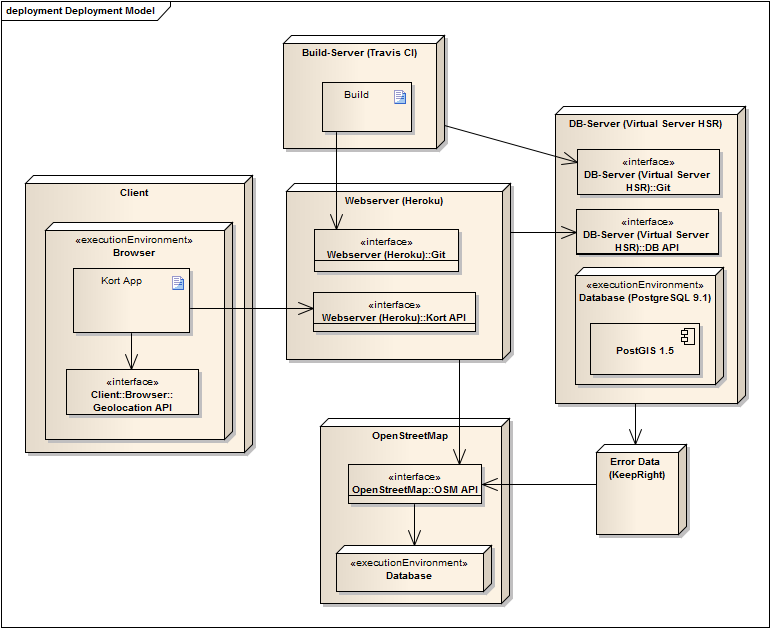
\includegraphics[width=\textwidth]{images/uml/deployment_diagram}
	\caption{Gesamtübersicht der Systeme}
	\label{deplyoyment-diagram}
\end{figure}


\section{Datenbankserver}

Beim Datenbankserver handelt es sich um einen virtuellen Server, den uns die Hochschule für Technik Rapperswil (HSR) zur Verfügung gestellt hat für die Dauer dieser Arbeit.

\begin{table}[H]
\centering
\begin{tabular}{|p{0.25\twocelltabwidth}|p{0.75\twocelltabwidth}|}
\hline 
\small{\textbf{Art des Servers}} & Virtueller Server \\
\hline 
\small{\textbf{Betriebsystem}} & Ubuntu 12.04 (LTS) \\
\hline 
\small{\textbf{Zugriff}} & Root-Zugriff via SSH \\
\hline 
\small{\textbf{Installierte Software}} & PostgreSQL 9.1, PostGIS 2.0, Redmine 2.1 \\
\hline 
\end{tabular} 
\caption{Datenbankserver der Hochschule für Technik Rapperswil}
\label{infrastruktur-datenbankserver-tabelle}
\end{table}

\subsection{Backup}
\todo[inline]{Backup-Section schreiben (DB-Server)}

\section{Webserver (Heroku)}

Bei Heroku\footnote{\url{http://www.heroku.com/}} handelt es sich um einen kostenlosen Dienst, welcher für verschiedenste Plattformen eine Deploymentumgebung anbietet. 
Der Dienst hat eine Schnittstelle über welche sich automatisiert Applikationen erstellen lassen, die Datenübertragung läuft dann über \gls{git}.

\begin{table}[H]
\centering
\begin{tabular}{|p{0.25\twocelltabwidth}|p{0.75\twocelltabwidth}|}
\hline 
\small{\textbf{Art des Servers}} & Server in der \gls{Cloud} \\
\hline 
\small{\textbf{Betriebsystem}} & Ubuntu \\
\hline 
\small{\textbf{Zugriff}} & Daten via \gls{git}, Befehle via Kommandozeilen-API (Heroku Toolbelt) \\
\hline 
\small{\textbf{Installierte Software}} & Apache, kort Applikation \\
\hline 
\end{tabular} 
\caption{Server bei Heroku}
\label{infrastruktur-heroku-tabelle}
\end{table}

Die Entscheidung den Webserver von Heroku zu wählen ist dadurch begründet, dass uns dies die grösstmögliche Freiheit bietet. 
Heroku bietet bereits eine hervoragende \gls{API} welche sich über das Kommandozeilen-Toolset \emph{Heroku-Toolbelt} steuern lässt.
Dies erlaubt es beliebig viele Applikationen automatisiert zu erstellen.
Auch für den Betrieb bietet das API viele Möglichkeiten zur Fernwartung an (SSH-Zugang, Logs, Prozessorauslastung).
Alle diese Faktoren zusammen ergeben die ideale Lösung für 

\section{Deployment}
Am Deployment der Applikation sind mehrere Systeme beteiligt. 
Alle Änderungen werden von den Entwicklern via \gls{git} zu GitHub\footnote{\url{http://github.com}} übertragen. 
Auf GitHub gibt es sogenannte Hooks die man aktivieren kann. 
Dabei handelt es sich um weitere Aktionen welche durch verschiedene Ereignisse ausgelöst werden können. 
In unserem Fall haben wir einen \emph{post-commit Hook} aktiviert, welcher dem \gls{ci} Dienst Travis-CI\footnote{\url{http://travis-ci.org}} Bescheid gibt, wenn ein neue Änderungen auf GitHub eingetroffen sind.

Auf Travis läuft dann der Build, welcher durch die Konfigurationsdatei \inlinecode{.travis.yml} gesteuert ist. Darin lassen wir die Schritte sowie die Umgebung für Builds definieren. Für jede Umgebung wird dann ein separater Build ausgelöst. Somit lassen sich bequem verschiedene Versionen mit unterschiedlichen Umgebungen testen.
Daraus entsteht dann eine sogenannte Build-Matrix welche bei jedem Build durchlaufen wird (siehe Tabelle \ref{infrastruktur-build-matrix}).

Ein Travis-Build läuft immer in einer neuen virtuellen Umgebung, so dass strikt nach dem Prinzip des \emph{\gls{Bootstrapping}s} vorgegangen werden muss. Das heisst, es muss möglich sein die Applikation ohne Vorkenntnisse zu installieren, alle benötigte Software und Konfiguration muss bei jedem Build vorgenommen werden.
Dies hilft, den Installationprozess genau festzuhalten

Am Ende des Build-Vorgangs wird die \gls{WebApp} schliesslich zu Heroku übertragen. 

\begin{table}[H]
\centering
\begin{tabular}{|p{0.2\threecelltabwidth}|p{0.4\threecelltabwidth}|p{0.4\threecelltabwidth}|}
\hline 
 & \textbf{Test} & \textbf{Produktion} \\
\hline 
\textbf{PHP 5.3} & Build und Test & Build und Test \\
\hline 
\textbf{PHP 5.4} & Build, Test und Deployment auf \url{http://kort-dev.herokuapp.com} & Build, Test und Deployment auf \url{http://kort.herokuapp.com} \\
\hline 
\end{tabular} 
\caption{Build-Matrix von Travis CI}
\label{infrastruktur-build-matrix}
\end{table}

\todo[inline]{gruntjs, ant, secure ENV, }
\todo[inline]{PHPDoc, PHPCS}
\todo[inline]{Update-Service}
